%!TeX root=MemoriaTFG.tex

\chapter{Introducción}
En plena era del dato \cite{Borkovich01}, la necesidad por obtener conocimiento a partir 
de gran cantidad de datos generados ha hecho que la cantidad de avances en este 
ámbito incremente notablemente. En la actualidad tenemos toda una serie de 
dispositivos: smartphones, smartwatches, pulseras deportivas, chalecos deportivos ..., 
que están generando información diversa del individuo que lo usa. La posición 
geográfica es una de las principales, seguida de información temporal, frecuencia 
cardíaca y un conjunto de información que puede ser tratada para obtener 
conocimiento sobre la población. 

La información del posicionamiento geográfico  de los individuos que los \ac{GIS} 
proporcionan constantemente hace que sea posible obtener, tratar, analizar y explotar 
dicha información. La explotación de estos datos puede llevarse a diferentes 
aplicaciones: puede ser usada para determinar la posición de un individuo, para 
sistemas de navegación en los que un individuo se desplaza desde un punto origen a 
un punto destino , la monitorización del movimiento de individuos, entre otras 
\cite{GPS01}. 

Una de las grandes utilidades de la explotación de estos datos consiste en el análisis de 
redes de caminos y carreteras, de forma que se puede obtener indicadores sobre el 
volumen de paso de individuos por caminos o carreteras, así como para la planificación 
de trayectorias, entre otros indicadores. Un ejemplo claro de esta utilidad es la 
explotación del dato para el conocimiento en el transporte.  Tanto en la forma en la que 
los individuos se trasladan al análisis de las carreras de un vehículo de transporte, tanto 
público como privado, como Uber o Cabify \cite{Viskic01}. En la figura 
\ref{figure:UberGL} se muestra un ejemplo, \textit{deck.gl}, un framework que permite 
la exploración visual de grandes volúmenes de datos. \cite{Uber01}.
\begin{figure}[!htb]
\begin{center}
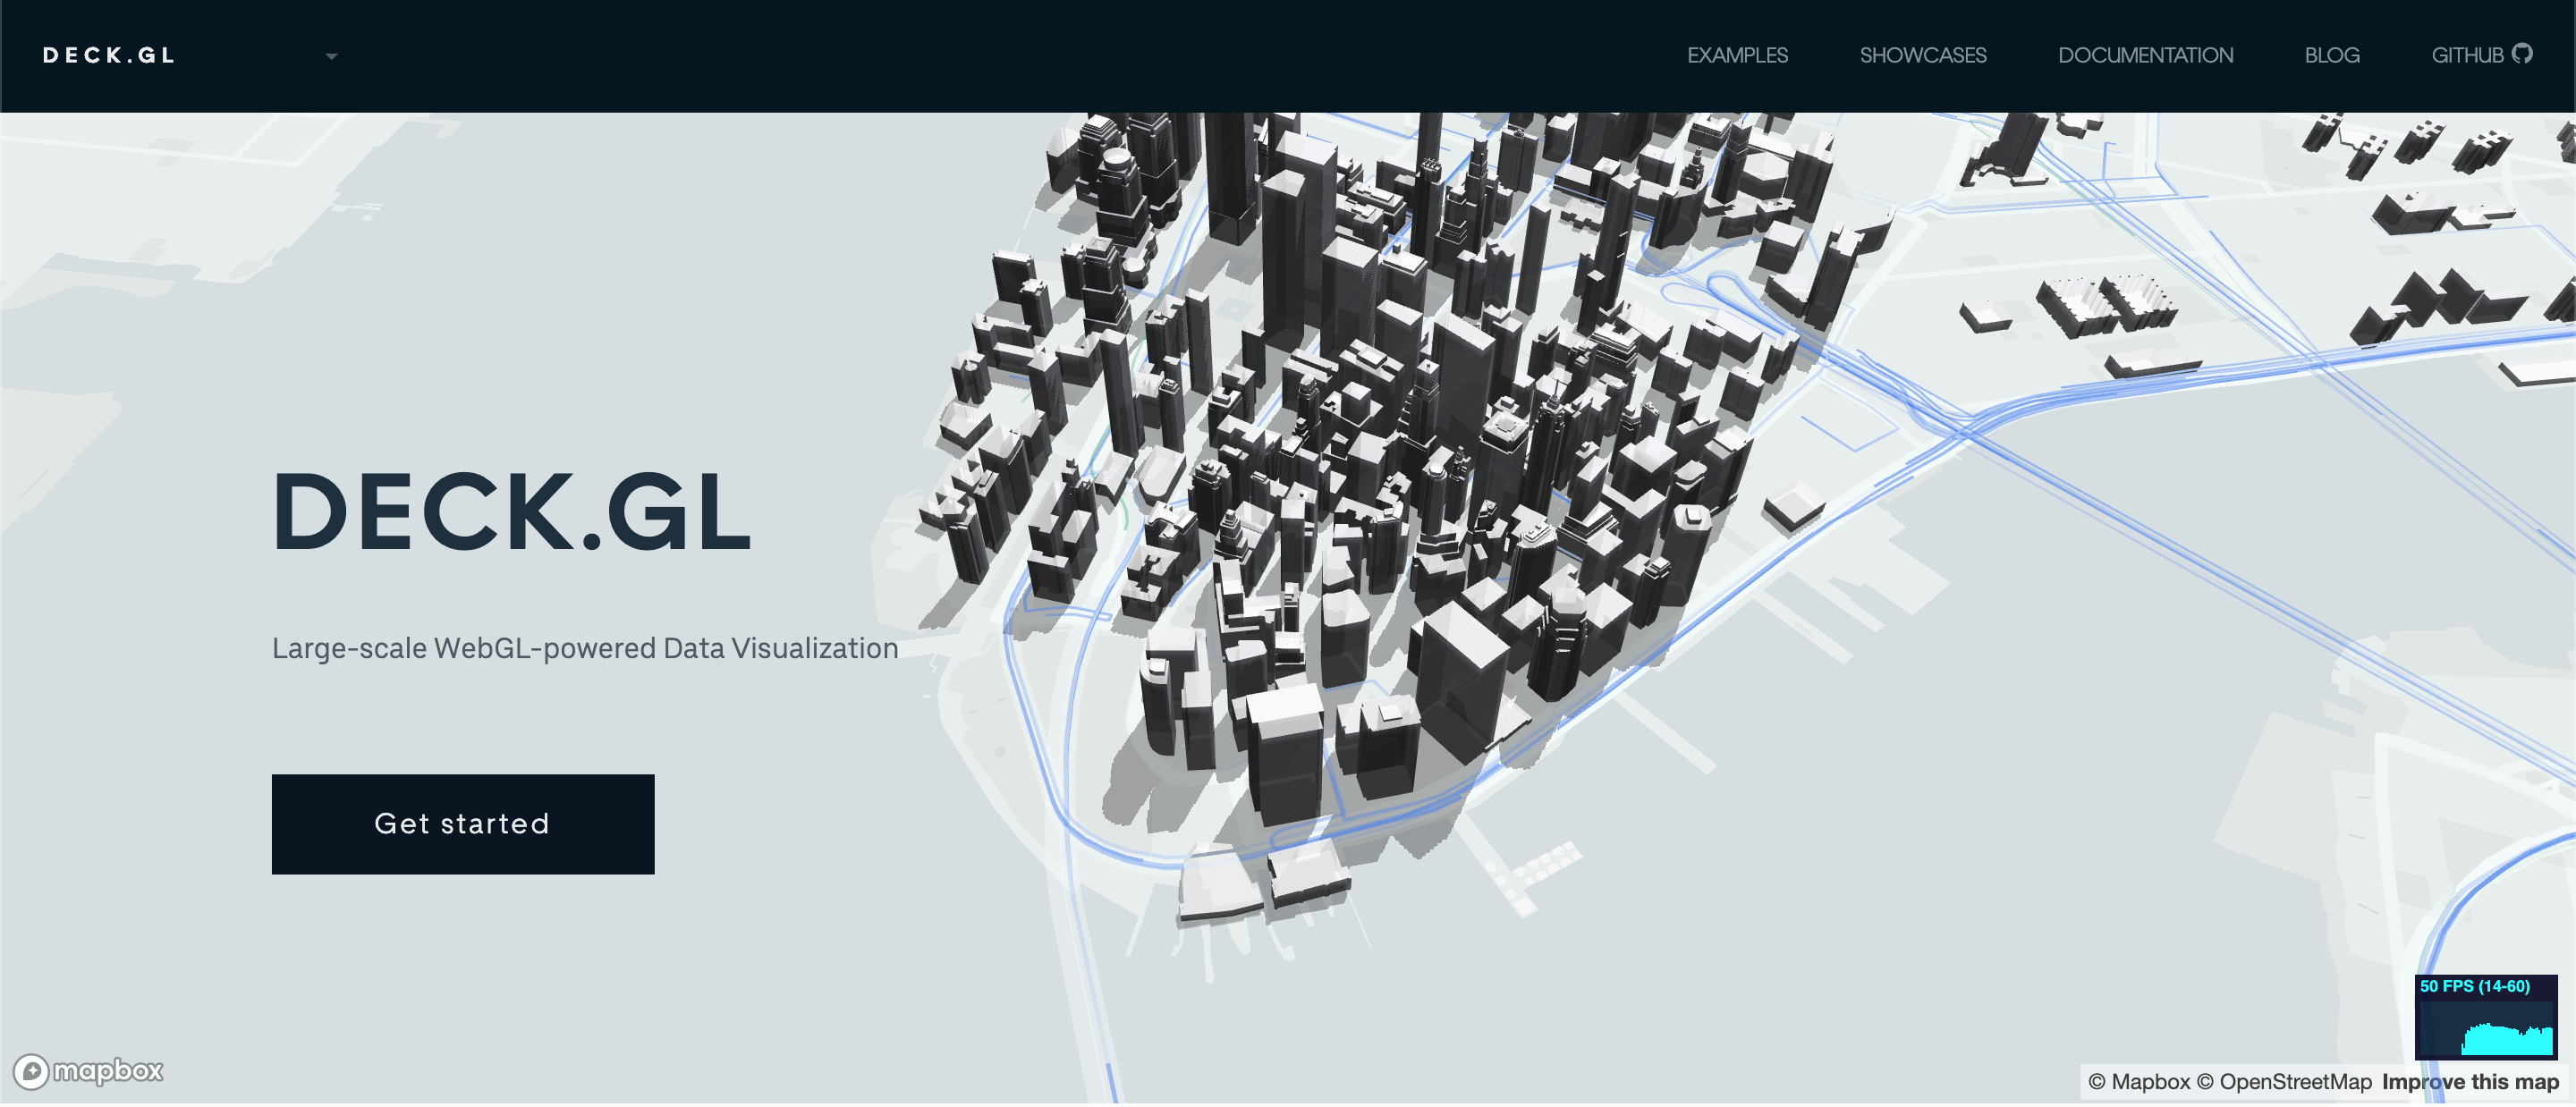
\includegraphics[width=0.9\textwidth]{./Imagenes/UberGL.png}
\caption{\textit{deck.gl}, proyecto de Uber.}
\label{figure:UberGL}
\end{center}
\end{figure}
\newpage
Es en este ámbito en el que aparece la necesidad de una herramienta que sea capaz de 
analizar la información que obtienen los diferentes \ac{GIS}, almacenar y transformar 
este conocimiento para poder generar trayectorias similares a la realidad dentro de un 
territorio geográfico conocido.

\textbf{\textit{track-simulator}} es una \ac{CLI}, propuesta en este documento, para la 
generación de trayectorias pseudo-aleatorias. \textit{track-simulator} cumple una serie 
de requerimientos que están descritos detalladamente en el capítulo 
\ref{chapter:AppArchitecture}. Estos requerimientos son:
\begin{enumerate}

\item Importación de datos en formato \ac{GPX}.

\item Análisis de trayectorias, obteniendo información medible y cuantificable.

\item Almacenamiento de las rutas reales y de los resultados del análisis en base de 
datos

\item Generación de fichero de gráficas resultantes del análisis 

\item Lectura de la base de datos para el acceso a la información

\item Simulación de puntos \ac{GPS}

\item Generación del fichero GPX correspondiente a la simulación de la trayectoria

\item Generación de fichero visualización de trayectoria

\end{enumerate} 

Esta propuesta está desarrollada en el lenguaje Python y utiliza diferentes librerías 
externas, entre las que se destaca \textbf{\textit{osmnx}} para el el análisis a partir del 
uso de redes de caminos y carreteras \cite{Boeing01}, \textbf{\textit{pandas}} para el 
tratamiento de datos \cite{Pandas01} y \textbf{\textit{gpxpy}} para la manipulación de 
ficheros \ac{GPX} \cite{Gpxpy01}. Estas, junto al resto de librerías externas utilizadas 
se describen en detalle en el capítulo \ref{chapter:AppArchitecture}.

La infraestructura de la aplicación está formada a partir de contendores de 
\textbf{Docker} \cite{Docker01}, de esta forma, la aplicación puede ser ejecutada en 
cualquier máquina que tenga Docker instalado, eliminándose cualquier tipo de 
problema que pueda surgir entre dependencias del aplicativo y la máquina en la que se 
ejecuta. Encontramos entonces dos contenedores: el primero contiene una conexión 
con una base de datos MongoDB, en la que almacena tanto las trayectorias analizadas 
como los resultados de los diferentes análisis. El segundo contenedor contiene el 
aplicativo \textit{track-simulator}. Este contenedor contiene todo el código, 
dependencias y configuración necesario para que el usuario pueda analizar un conjunto 
de trayectorias almacenadas en ficheros  \ac{GPX}. Este análisis lo hace a partir de una 
técnica llamada \textit{map-matching} consistente en unir los datos con la red lógica 
de caminos y carreteras.

Después de la etapa de análisis, el usuario puede realizar una generación de 
trayectorias. Estas son generadas de forma pseudo-aleatoria a partir de la información 
analizada en la anterior etapa. Cada trayectoria generada es única en si misma y replica 
el comportamiento de los individuos analizados.

Finalmente como productos resultantes de esta herramienta encontramos ficheros con 
la información resultante del análisis del conjunto de trayectorias, así como ficheros 
\ac{GPX} y representaciones gráficas de las trayectorias simuladas.

Este documento se compone de 8 capítulos donde aparecen 3 diferentes bloques: el 
primer bloque  (capítulo \ref{chapter:PrincipalConcepts} y 
\ref{chapter:AppArchitecture}   serían la introducción al problema y la arquitectura de la 
herramienta. Del capítulo \ref{chapter:DataAnalysis} al \ref{chapter:Experimentation} se 
explican los diferentes módulos que componen el aplicativo y el flujo de los datos, 
explicando detalladamente el análisis de los datos y el algoritmo de simulación de las 
trayectorias, cerrando el bloque con una muestra de los resultados la experimentación 
del aplicativo. Finalmente el capítulo \ref{chapter:GuiaUso} explica al lector como 
instalar y usar la herramienta. El capítulo \ref{chapter:Conclusion} cierra el documento 
con las opiniones finales.

Los capítulos son los siguientes:

\begin{enumerate}[label={C. \arabic*.}]
\setcounter{enumi}{1}
\item \textbf{Conceptos principales}. Capítulo introductorio al lector. Aparecen los 
conceptos básicos y las herramientas conocidas dentro del marco del tratamiento de 
datos \ac{GPS}.

\item \textbf{Arquitectura de la aplicación}. Descripción de las funcionalidades que 
componen la propuesta. Flujo de datos de la herramienta y requerimientos básicos que 
cumple. Se muestra al lector la estructura de \textit{track-simulator} y el problema que 
resuelve.

\item \textbf{Análisis de los datos \ac{GPS}}. Capítulo donde se explica detalladamente 
como se analiza el dato. Desde la preparación del entorno hasta la explotación del dato, 
pasando detalladamente por el proceso de definición de heurísticas y parámetros.


\item \textbf{Simulación de trayectorias}. Explicación del proceso de generación de 
trayectorias pseudo-aleatorias. De define la forma en la que se generan 
individualmente los puntos \ac{GPS}. Se muestra la implementación técnica 
destacable.

\item \textbf{Experimentación}. Muestra de resultados del uso de la herramienta. Se 
realizan dos experimentaciones: con introducción de datos analizados y sin 
introducción de datos. Se muestran gráficas comparativas y se comentan en detalle los 
resultados.

\item \textbf{Guía de instalación y uso}. Conjunto de pasos a seguir para instalar el 
aplicativo en una máquina. En ese capítulo se explican instrucciones disponibles y los 
parámetros necesarios para su ejecución, completando con ejemplos.

\item \textbf{Conclusión}. Capítulo de cierre del documento y de la propuesta. Se 
describe el futuro del aplicativo, así como la opinión personal del desarrollo del 
proyecto. Se concluye la propuesta.
\end{enumerate}